\chapter{Typ-III Remailer}
Die als Typ-II klassifizierten Mixmaster-Remailer gelten in der Praxis als sicher. Trotzdem wurde das Mixminion-Remailer Protokoll entworfen. Mixminion-Remailer stellen den Typ-III der Remailerklassifizierung dar. Die signifikanten Neuerungen, die mit dem Mixminion-Remailer Protokoll eingeführt wurden, waren:
\begin{itemize}
\item das Antworten auf anonyme Nachrichten
\item verschlüsselte Kommunikation zwischen den Remailern (TLS statt SMTP)
\item Einführung einer Verzeichnisserverstruktur
\item automatischer Schlüsselwechsel nach definiertem Intervall
\end{itemize}

Die Möglichkeit auf eine empfangene anonyme Nachricht zu antworten, ist der entscheidende Vorteil der Mixminion-Remailer. Kein anderes anonymisierendes Remailer Protokoll (Typ-I und Typ-II) unterstützt dieses Feature nativ.

Die Mixminion-Remailer sind, äquivalent zu den vorherigen Remailer Protokollen, eine Weiterentwicklung des vorherigen Protokolls. So bilden die Mixmaster-Remailer die technische Grundlage für die Entwicklung des Mixminion Protokolls.

\section{Funktionsweise}
\subsection{SURBs}
Die Single-Use-Reply-Blocks\footnote{kurz: SURBs.} wurden eingeführt, um dem Empfänger das Antworten auf eine empfangene anonyme Nachricht zu ermöglichen. Dabei soll die Anonymität des  Senders erhalten bleiben.

Betrachtet man die Lage basierend auf den vorherigen Remailer-Protokollen, kann Bob nicht auf eine über ein Remailer-Netzwerk versandte Nachricht von Alice antworten. Das liegt daran, dass ihm lediglich die Identität des letzten Remailers bekannt ist, nicht jedoch die von Alice.

Um Bob ein Antworten zu ermöglichen, erstellt Alice einen Single-Use-Reply-Block und hängt diesen an die Nachricht an. Der SURB befindet sich dabei in verschlüsselter Form im Header der Nachricht. 
Ein SURB enthält zwei wichtige Informationen:
\begin{itemize}
\item die E-Mail Adresse von Alice in verschlüsselter Form
\item einen Pfad durch das Remailer-Netzwerk zu Alice
\end{itemize}

Wichtig ist, dass der SURB für den Empfänger nicht entschlüsselbar ist. Bob ist weiterhin nicht in der Lage die Identität von Alice zu entschlüsseln. Dazu ist lediglich der entsprechende Mixminion-Remailer fähig. Bob kann jedoch den SURB dazu verwenden, um Alice auf ihre anonyme Nachricht zu antworten. Dazu hängt Bob seine Antwortnachricht an den SURB an und verschickt dieses Konstrukt an den ersten Remailer des im SURB vorhandenen Remailerpfades. Der letzte Remailer dieses Pfades kann die Adresse von Alice entschlüsseln und die Antwort an Alice weiterleiten.

Bob kann pro empfangenen SURB nur eine Nachricht an Alice schicken. Das liegt darin begründet, dass ein SURB nur einfach verwendbar ist.\footnote{daher SINGLE-USE-Reply-Block.} Möchte Bob Alice eine weitere Nachricht schicken, muss er auf eine weitere Nachricht von Alice warten, die einen SURB enthält, um diesen für eine erneute Antwort zu verwenden. Nach der einmaligen Verwendung eines SURBs werden alle weiteren Nachrichten, die mit Hilfe dieses SURBs versendet werden, wie Duplikate betrachtet und verworfen.

\subsection{Nachrichten}
\subsubsection{Typisierung}
Bisher existierte in den Remailer-Protkollen nur eine Art von Nachricht -- eine anonyme Nachricht von Alice an Bob. Für die Hinzunahme von Antwortnachrichten, die gesondert behandelt werden müssen, ist die Einführung einer Typisierung von Nachrichten für das Mixminion-Remailer Protokoll unerlässlich. Hierbei wird zwischen drei Arten von Nachrichten unterschieden:\footnote{vgl. S. 4 \cite{mixminion}.}

\begin{enumerate}
\item normale Nachrichten
\item direkte Antworten über SURBs
\item anonyme Antworten
\end{enumerate}

Eine normale Nachricht entspricht einer anonymisierten Nachricht von Alice an Bob, wie sie aus den bisherigen Protokollen bekannt ist. Bei einer direkten Antwort über einen SURB gibt Bob bei der Antwort seine Identität preis. Da er nicht weiß, ob er wirklich Alice antwortet -- denkbar wäre auch, dass Alice die Adresse eines Dritten in dem SURB angegeben hat -- ist es wünschenswert, dass Bob ebenfalls die Möglichkeit hat bei einer Antwort anonym zu bleiben.\footnote{das ist nur ein beispielhafter Grund. Logischerweise könnte Bob auch aus anderen Gründen anonym bleiben wollen.} Hierfür existiert die dritte Art einer Nachricht, bei der die Identität von Bob ebenfalls verborgen wird.

\subsubsection{Ununterscheidbarkeit}
In den vorherigen Kapiteln wurde darauf hingewiesen, dass es für die Gewährleistung der Sicherheit unerlässlich ist, dass der Datenverkehr innerhalb des Remailernetzwerks für Eve transparent erscheinen muss. Eve darf nicht dazu in der Lage sein, durch die Analyse des Datenverkehrs eine Verbindung zwischen einkommenden und ausgehenden Nachrichtenvekehr herstellen zu können.

Dieser Zustand muss auch nach der Einführung verschiedener Nachrichtentypen erhalten bleiben.  Die Nachrichtentypen müssen daher nach außen hin ununterscheidbar sein. Das ist wichtig, damit Eve keine Rückschlüsse bezüglich der Art des Nachrichtenverkehrs über die Unterscheidung der Nachrichtentypen ziehen kann. Diese Transparenz wird dadurch gewährleistet, dass alle drei Nachrichtenarten strukturell identisch aufgebaut sind. Sie verfügen über gleichgroße Header- und Bodygrößen.\footnote{Body wird häufig auch Payload genannt.}

\subsubsection{Strukturen der unterschiedlichen Typen}
Die Nachrichten die in einem Mixminion-Remailer Netzwerk verschickt werden, sind ingesamt 32kB groß. Durch diese Gleichförmigkeit der Größe liefert eine Analyse des Traffic keinen Aufschluss darüber, welche Arten von Nachrichten gerade in dem Remailer-Netzwerk ausgetauscht werden.

Jede Nachricht im Mixminion-Protokoll besteht grundlegend aus den Komponenten 
\begin{itemize}
\item Header
	\begin{itemize}
	\item primärer Header
	\item sekundärer Header
	\end{itemize}
\item Body (Payload)
\end{itemize}

Signifikant ist, dass der Header sich in zwei Teile aufteilt -- dem primären und dem sekundären Header. Dabei haben der primäre und der sekundäre Header jeweils eine Größe von 2kB und der Body eine Größe von 28kB. Der Body einer Nachricht enthält, unabhängig vom Typ der Nachricht, die eigentlich zu übertragende Information; im letzten Schritt also die Nachricht des Senders an den Empfänger. Die Typisierung einer Nachricht wird durch den Inhalt des primären und sekundären Headers unterschieden.

\begin{figure}
	\begin{center}
		\def\svgwidth{0.9 \linewidth}
		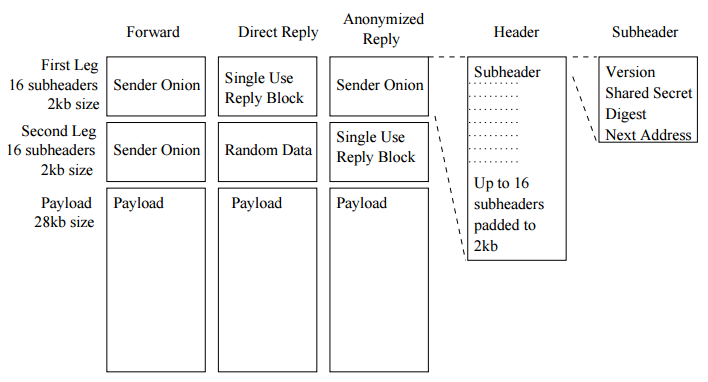
\includegraphics[width = 0.9 \linewidth]{bilder/mixminion_structure.png}
		\caption{Die Nachrichtenstruktur im Mixminion-Protokoll}
		\caption*{\hfill Source: S. 4 \cite{mixminion}.}
	\end{center}
\end{figure}

Die obige Abbildung beschreibt den Inhalt des primären und des sekundären Headers in den verschiedenen Nachrichtenfällen.
Man sieht, dass sowohl der primäre als auch der sekundäre Header im Fall einer normalen Nachricht, als auch der primäre Header im Falle einer anonymen Antwort, Pfadinformationen durch das Netzwerk beinhalten.
Ein solcher Pfad ist in Subheader aufgeteilt. Jeder Subheader entspricht einem Datum für den nächsten Remailer des Pfades und beinhaltet im wesentlichen drei Daten:
\begin{itemize}
\item ein Master-Secret für die Erstellung eines symmetrischen Schlüssels für den Aufbau einer verschlüsselten Verbindung zum nächsten Remailer im Pfad
\item eine Adresse des nächsten Remailers im Pfad
\item eine Prüfsumme zum Überprüfen der Integrität des Rests des Headers
\end{itemize}
Die Pfade des primären und sekundären Headers ergeben, im Falle einer normalen Nachricht, zusammen den Gesamtpfad der Nachricht durch das Remailernetzwerk zum Empfänger. Dabei entspricht der Pfad im primären Header dem ersten Teil, der Teil im sekundären Header dem zweiten Teil des Pfades.
Sowohl der primäre als auch der sekundäre Header können sich maximal aus 16 dieser Subheader zusammensetzen. Demzufolge ist die maximale Länge der Route einer normalen Nachricht im Mixminion-Protokoll 32.

Bei einer direkten Antwort von Bob ist der SURB im primären Header der, der von Alice zum Antworten übermittelt wurde. Da in diesem alle Informationen enthalten sind, die benötigt werden um die Nachricht bis zu Alice durchzustellen, befinden sich im sekundären Header in diesem Fall keine signifikanten Informationen. Um den gleichartigen Schein zu wahren, wird der sekundäre Header mit Platzhalterdaten gefüllt.

Bei einer anonymen Antwort befindet sich der SURB von Alice im sekundären Header. Im primären Header befindet sich ein von Bob spezifizierter Pfad durch das Netzwerk, der vor dem Pfad des SURBs durchlaufen wird. Dadurch bleibt die Identität von Bob dem Empfänger der Antwort verborgen.\footnote{vgl. S. 4 \cite{mixminion}.}

\subsection{Verzeichnisserver}
Eine weitere Neuerung im Mixminion-Protkoll ist die Einführung von Verzeichnisservern. Ein Verzeichnisserver trägt für jeden Mixminion-Remailer im Netzwerk drei unmittelbar relevante Informationen:\footnote{vgl. S. 8 \cite{mixminion}.}
\begin{itemize}
\item Die Existenz eines Remailers
\item Den aktuellen Schlüssel des Remailers
\item Den aktuellen Status des Remailers
\end{itemize}

Alle drei Eigenschaften werden den Verzeichnisservern von den Remailern selbst mitgeteilt.
Wichtig ist, dass es nicht nur einen Verzeichnisserver pro Netzwerk gibt. Pro Netzwerk gibt es mehrere Verzeichnisserver. Diese verschiedenen Verzeichnisserver müssen dauerhaft synchronisiert sein, damit sichergestellt ist, dass sie die gleichen Daten bezüglich des Remailernetzwerks verteilen (Redundanz). Dadurch wird auch verhindert, dass nicht funktionstüchtige Remailer weiter von einem Benutzer in deren Nachrichtenpfad eingebaut werden. Dies würde dazu führen, dass eine Nachricht nie ihren Empfänger erreichen würde. Des weiteren haben die Verzeichnisserver die Aufgabe, sich dauerhaft gegenseitig zu verifizieren. Dadurch wird verhindert, dass ein Angreifer einen manipulierten Verzeichnisserver einspielt, um beispielsweise alle Daten nur über bestimmte Remailer laufen zu lassen.\footnote{vgl. S. 9 \cite{mixminion}.} Bei dieser Vorgehensweise wird davon ausgegangen, dass nicht alle Verzeichnisserver manipuliert sind, da ansonsten die gegenseitige Verifikation und Synchronisation hinfällig wäre.

\section{Ablauf}
Möchte Alice eine Nachricht an Bob senden, benötigt sie zunächst alle nötigen Informationen vom Verzeichnisserver. Von diesem erhält sie den Status und die relevanten aktuellen Schlüssel zu jedem Remailer im Netzwerk. Die schichtweise Verschlüsselung der Nachricht erfolgt äquivalent zum Mixmaster Protokoll. Zusätzlich wird der sekundäre Header mit der Prüfsumme des Nachrichtenbodies verschlüsselt.
Anschließend sendet Alice die Nachricht an den ersten Remailer im Pfad.

Hat ein Remailer eine Nachricht empfangen und sein Puffer ist soweit gefüllt, dass er die Nachricht versenden möchte, wird zunächst die Integrität der Daten über die im Subheader angegebene Prüfsumme überprüft. Anschließend baut er mit Hilfe des ebenfalls im Subheader angegebenen Master-Secrets eine TLS-Verbindung zum nächsten Remailer im Pfad auf. Nachdem der Remailer die Nachricht entsprechend der schichtenweisen Verschlüsselung entschlüsselt hat überprüft er über die im Header angegebene Idenfitikation, ob die selbe Nachricht bereits behandelt wurde. Ist die Überprüfung erfolgreich überträgt er die Nachricht, ansonsten wird die Nachricht verworfen. Danach wird die gesicherte Verbindung wieder aufgelöst.

Zur Überprüfung der Identifikation muss ein Remailer alle IDs der Nachrichten speichern, die er bereits behandelt hat. Dieser Speicher wird zum Zeitpunkt des Schlüsselwechsels geleert, da Nachrichten, die mit dem alten Schlüssel verschlüsselt wurden, zu diesen Zeitpunkt nicht mehr behandelt werden können. So wird einerseits verhindert, dass zu alte Nachrichten das Remailernetzwerk durchlaufen können, andererseits wird die Größe des Puffers auf diese Weise endlich gehalten.

Der Zeitpunkt, an der der gesamte Pfad des primären Headers durchlaufen ist, wird \glqq Crossover\grqq -Punkt genannt. An diesem Punkt wird der sekundäre Header mit Hilfe der Prüfsumme des Nachrichtenbodies entschlüsselt und der primäre mit dem sekundären Header vertauscht.\footnote{dieser Vorgang wird als swap operation bezeichnet. Vgl. S. 4-5 \cite{mixminion}.} Wurde eine Nachricht in der Zwischenzeit manipuliert, ändert sich die Prüfsumme des Nachrichtenbodies und der sekundäre Header ist nicht entschlüsselbar. In diesem Fall wird die Nachricht verworfen.\footnote{vgl. S. 5 \cite{mixminion}.} Dadurch werden Attacken verhindert, die über eine Manipulation der Nachricht erfolgen. Nachdem der sekundäre Header erfolgreich entschlüsselt und entsprechend vertauscht wurde, wird wie im vorherigen Ablauf weiterverfahren, bis Bob die gesamte Nachricht empfängt. 

\section{Sicherheitsanalyse}
In der Theorie handelt es sich beim Mixminion-Protokoll um das sicherste der drei Remailer-Protokolle. Beim Entwurf wurden neuste Forschungsergebnisse und durch die älteren Remailer-Protokolle gesammelte Erfahrungen genutzt, um Schutzmechanismen gegen bekannte Angriffe zu realisieren.\footnote{vgl. S. 5ff \cite{mixminion}.} Ebenso wurden viele Mängel der früheren Remailer herausgearbeitet und beseitigt. 

Das Mixminion Protokoll ist jedoch nie in einem vollständigen Zustand implementiert worden. Es ist nie über die Beta-Phase der Implementierung hinaus gekommen. So existieren unter Umständen noch Fehler in der Implementierung, die die Sicherheit gefährden. Außerdem laufen viele Mixminion-Remailer aufgrund ihrer unfertigen Implementierung noch mit Debug-Einstellungen, sodass Aktivitäten geloggt werden. Dieser Zustand ist zu unsicher, sodass das Protokoll in der Praxis nicht aktiv genutzt wird. Daher konnten bisher keine praktischen Erfahrungen bezüglich der Sicherheit dieses Remailer-Protokolls gesammelt werden.


